\section{Introduction}

% (1) Introductory paragraph: Very briefly: What is the problem and why is it relevant to the audience attending *THIS CONFERENCE*? Moreover, why is the problem hard, and what is your solution? You must be brief here. This forces you to boil down your contribution to its bare essence and communicate it directly.
Conveying the behaviors of a dynamic system is extremely important in the field of robotics.
%
When presenting the operation of a new robotic system, it is vital to provide readers and collaborators with some way to visualize its motions.
%
This is particularly true for evolutionary robotics (ER) research, as
%
often the goal of ER is to produce \emph{novel} or unexpected behaviors.
%
Despite this importance, however, it can be difficult to present behaviors in a manner useful to other researchers.
%
In this paper, we present \textbf{Review}\footnote{https://review.github.io/} (source code\footnote{\url{https://github.com/review/review.github.io}}), a web-based platform for sharing visualizations of evolved robotic systems.




% (2) Background paragraph: Elaborate on why the problem is hard, critically examining prior work, trying to tease out one or two central shortcomings that your solution overcomes.
Traditionally, to depict behaviors of an evolved system, researchers provide sequences of images (see Figures~\ref{fig:quad_gaits} and~\ref{fig:worm_gaits}) and/or links to videos.
%
Image sequences have been a common feature of ER from the beginning; see, \textcite{Sims.1994.CGIT.Creatures} from \citeyear{Sims.1994.CGIT.Creatures} for example.
%
Images, however, can sometimes be problematic. First, when a reader is unfamiliar with terminology (\eg{}, gait, hopping, bounding, etc.) they may not have a baseline reference with which to compare and understand images of a new behavior.
%
And second, even with a good understanding of what to expect, some complex movements are difficult to comprehend from image sequences.
%
For example, the quadruped gaits in Figure~\ref{fig:quad_gaits} are reasonably understandable for someone familiar with such systems, but for someone new to quadrupedal robotics it may be difficult to picture the motions.
%
Likewise, the unusual gaits exhibited by the worm-like animat in Figure~\ref{fig:worm_gaits} are difficult to imagine without the aid of video (or animation).



\begin{figure*}[htb!]
\centering
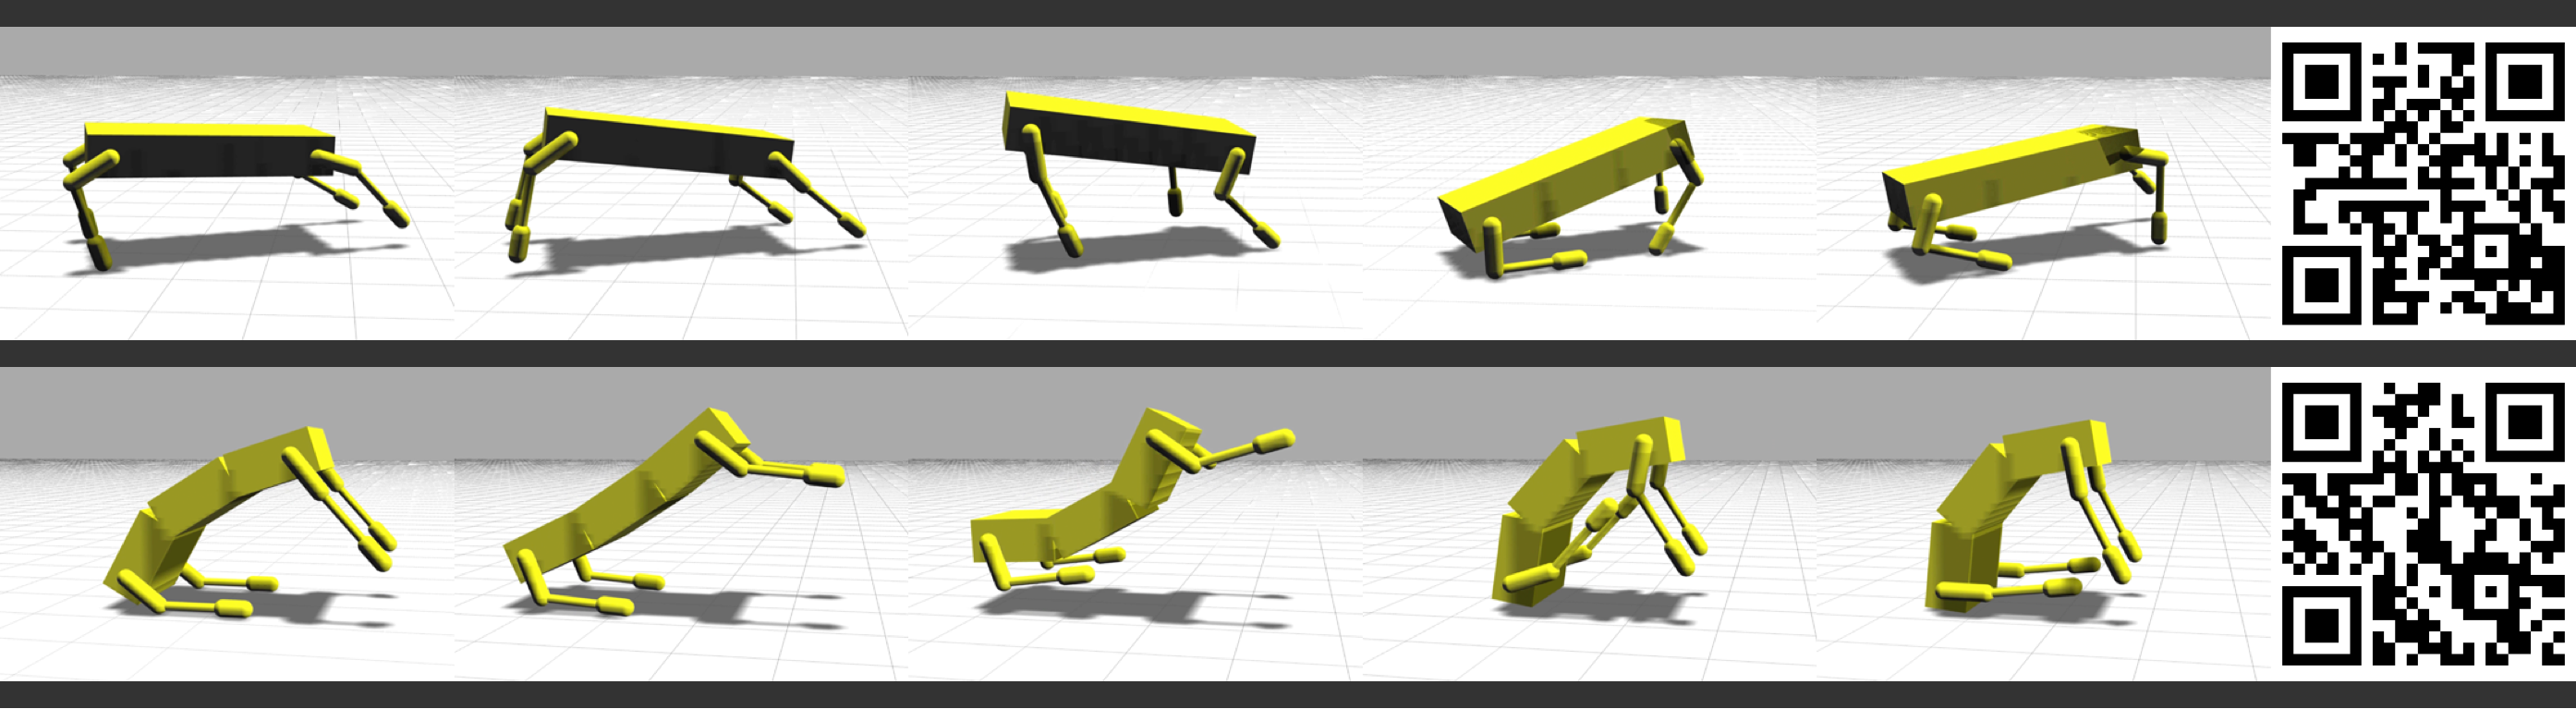
\includegraphics[width=\textwidth]{figures/quadruped.png}
\caption{Evolved gaits for a quadrupedal animat: (top) galloping, (bottom) hopping. Interactive visualizations of the galloping and hopping gaits can be found, respectively, at the following links: \url{http://bit.ly/2HYXS7u} and \url{http://bit.ly/2HVY9bc}; or by visiting the links specified by the QR codes.}
\label{fig:quad_gaits}
\end{figure*}

\begin{figure*}[htb!]
\centering
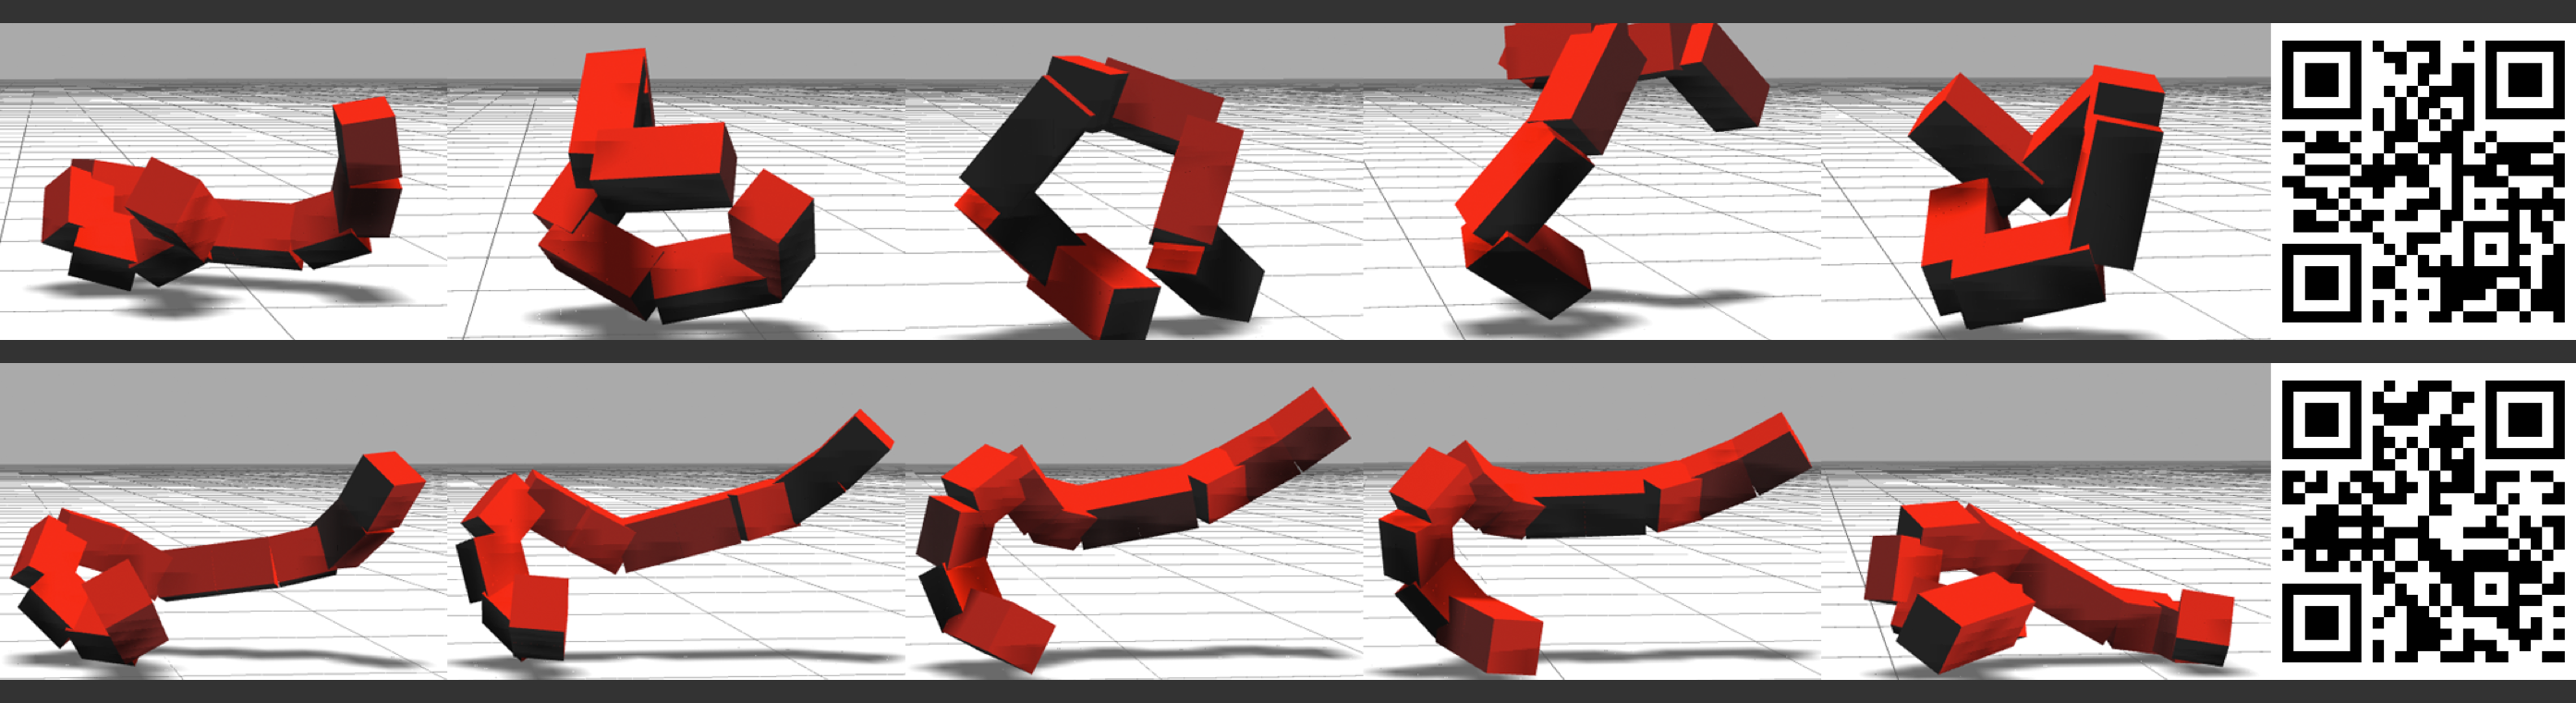
\includegraphics[width=\textwidth]{figures/worm.png}
\caption{Evolved gaits for a worm-like animat (adapted with permission from \textcite{Moore.2017.GECCO.Animat}): (top) tumbling, (bottom) hopping. Interactive visualizations of the tumbling and hopping gaits can be found, respectively, at the following links: \url{http://bit.ly/2vH4Knp} and \url{http://bit.ly/2HnHa4C}; or by visiting the links specified by the QR codes.}
\label{fig:worm_gaits}
\end{figure*}


Linking to videos is a common approach to handling the problems associated with images.
%
Videos, however, are similarly static in the sense that the camera transform (viewing angles, zoom levels, etc.), object materials (colors and other material properties), and playback speed are fixed once the video is generated and uploaded.
%
Practically, this means that a viewer of the video cannot change the view angle or zoom-in on different aspects of the scene, and cannot change the color of objects if they find the chosen colors hard to see.
%
And although some web-based video players allow a viewer to speed-up/slow-down the video by small amounts, this is usually at the cost of playback smoothness; videos appear \emph{choppy} when they are slowed down since videos are recorded at a fixed frame-rate and slowing down the video effectively makes each frame appear for a longer period of time.
%
Additionally, it is common for ER researchers to generate videos by performing a video screen recording (often referred to as a screencast).
%
Since the speed of a simulation playback depends on the current load of both the CPU and GPU, recording a simulation playback via screencasting generally leads to videos with irregular frame-rates.
%
Animation software, such as Review, does not have these drawbacks.




% (3) Transition paragraph: What keen insight did you apply to overcome the shortcomings of other approaches? Structure this paragraph like a syllogism: Whereas P and P => Q, infer Q.
Review was originally developed to share visualizations among colleagues.
%
Essentially, a tool was needed to solve two common questions in evolutionary robotics: (1) how can we share behavior results without needing to generate and email (or upload) large video files, and (2) how can we enable collaborators to manipulate the scene's camera as the visualization is playing.
%
One method for achieving these two goals is to setup the same simulation and graphics environment on the machines of all collaborators, such that everyone is able to repeat the same experiment when given the same configuration (\ie{}, control and morphology parameters and environment initial conditions).
%
To ensure repeatable results, in ER research this would require all collaborators to install the same physics and graphics libraries.
%
This works for small teams and simple software packages, however, it becomes untenable when dealing with more complex systems.




% (4) Details paragraph: What technical challenges did you have to overcome and what kinds of validation did you perform?
Instead, Review has the ability to playback visualizations, inside a browser, when provided a log file.
%
Thus, the work-flow works as follows: (1) a researcher runs an evolutionary experiment (likely with the aid of a compute cluster), (2) interesting solutions are re-run, with visualization logging enabled (see section~\ref{sec:review} for details), to generate log files, (3) log files are shared with other researchers (\eg{}, via email or uploaded to a website), and (4) log files are run with Review so that everyone can see the same results.
%
Importantly, everyone using Review can independently adjust the playback speed, color of objects, and camera.



% (5) Assessment paragraph: Assess your results and briefly state the broadly interesting conclusions that these results support. This may only take a couple of sentences. I usually then follow these sentences by an optional overview of the structure of the paper with interleaved section callouts.
Review is meant to be complementary to both image sequences and videos.
%
Many researchers will not have access to the Internet while reading a research paper, and for many other cases video will suffice.
%
A web-based simulation viewer is meant for the following scenarios:

\begin{enumerate}
    \item sharing research with collaborators that need the ability to examine the scene from their own perspective, and
    \item sharing difficult-to-visualize behaviors in such a way that readers can manipulate the camera to better understand evolved behaviors.
\end{enumerate}
